\section{Methodology}\label{method}
Remove the weekly trend of the data to analyze the detailed changes that convey the device behavior at small time scales.

\subsection{Empirical Mode Decomposition}

Empirical Mode Decomposition (EMD) \cite{huang:emd1998} is a recent techniques used for de-treding...

non-stationary non-linear signal

TODO explanation of EMD


intrinsic mode functions (IMFs)

In order to ensure that the IMFs corresponding to two distinct signals the EMD decomposition is 
We use bivariate EMD \cite{rilling:biemd2007} to decompose two signals at once and obtain their IMF at the same time scale.

\begin{figure*}
 \subfigure[EHP vs. Light]{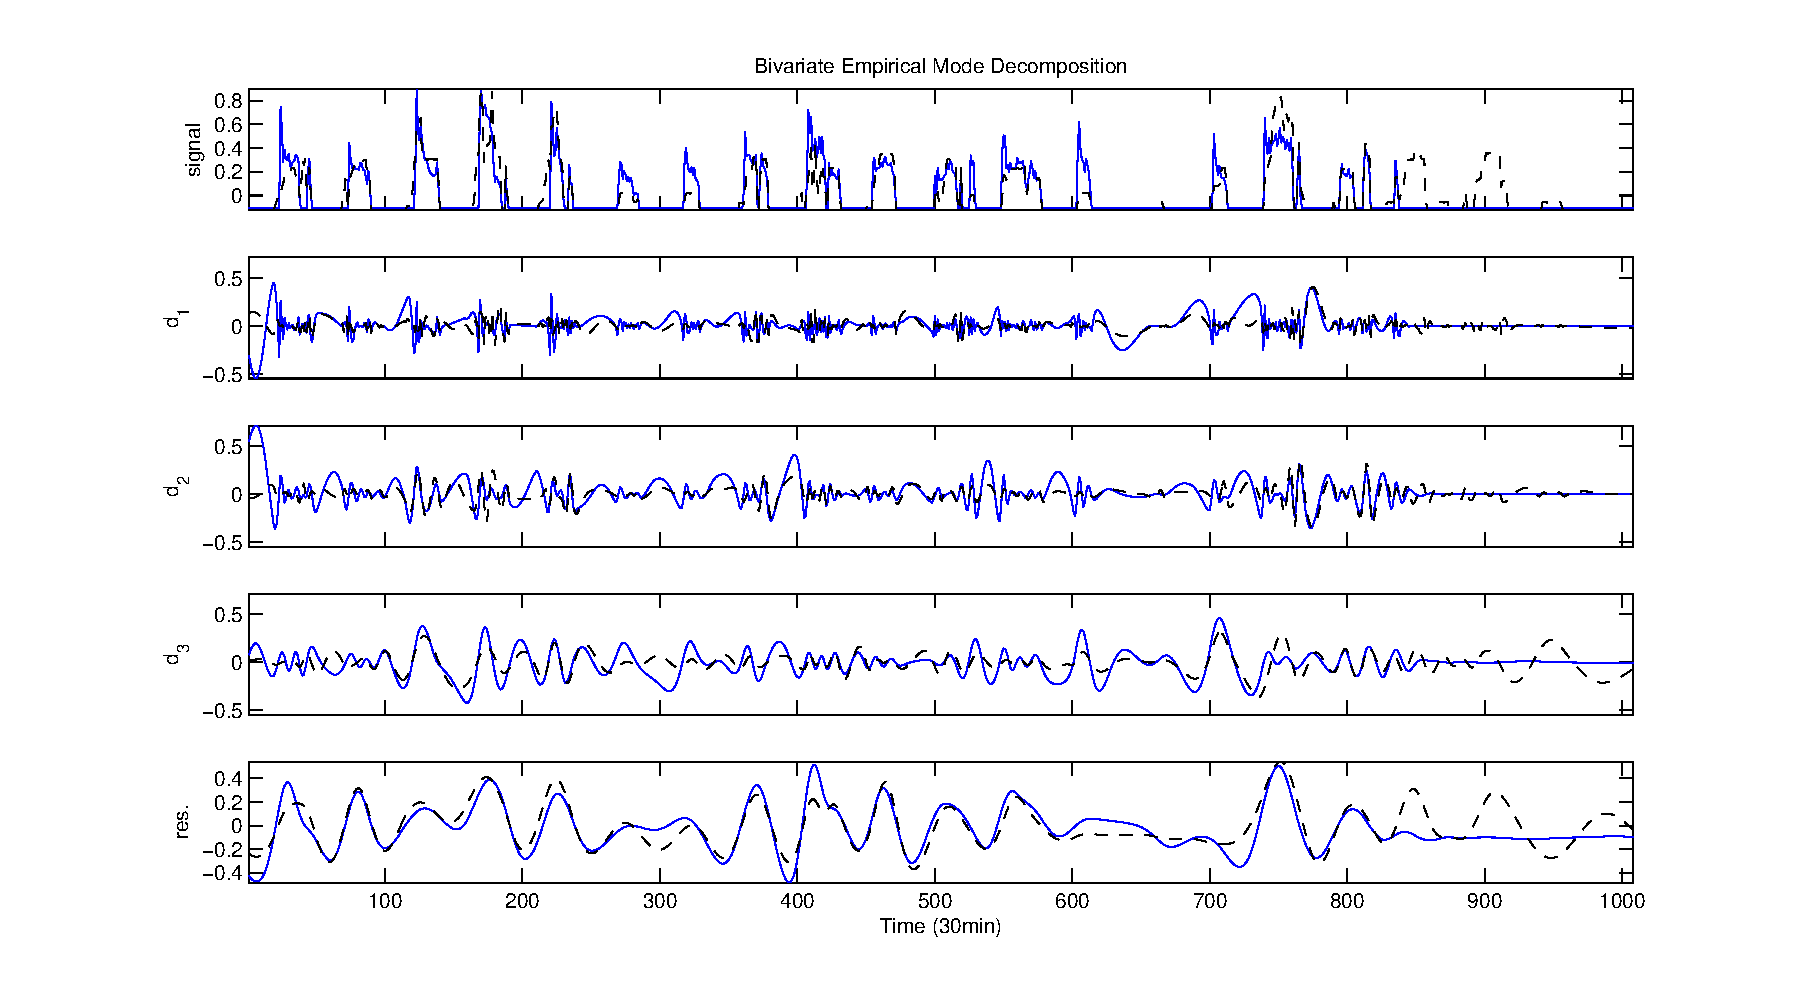
\includegraphics[width=\textwidth]{img/emd_25_26}}
 \subfigure[EHP vs. GHP]{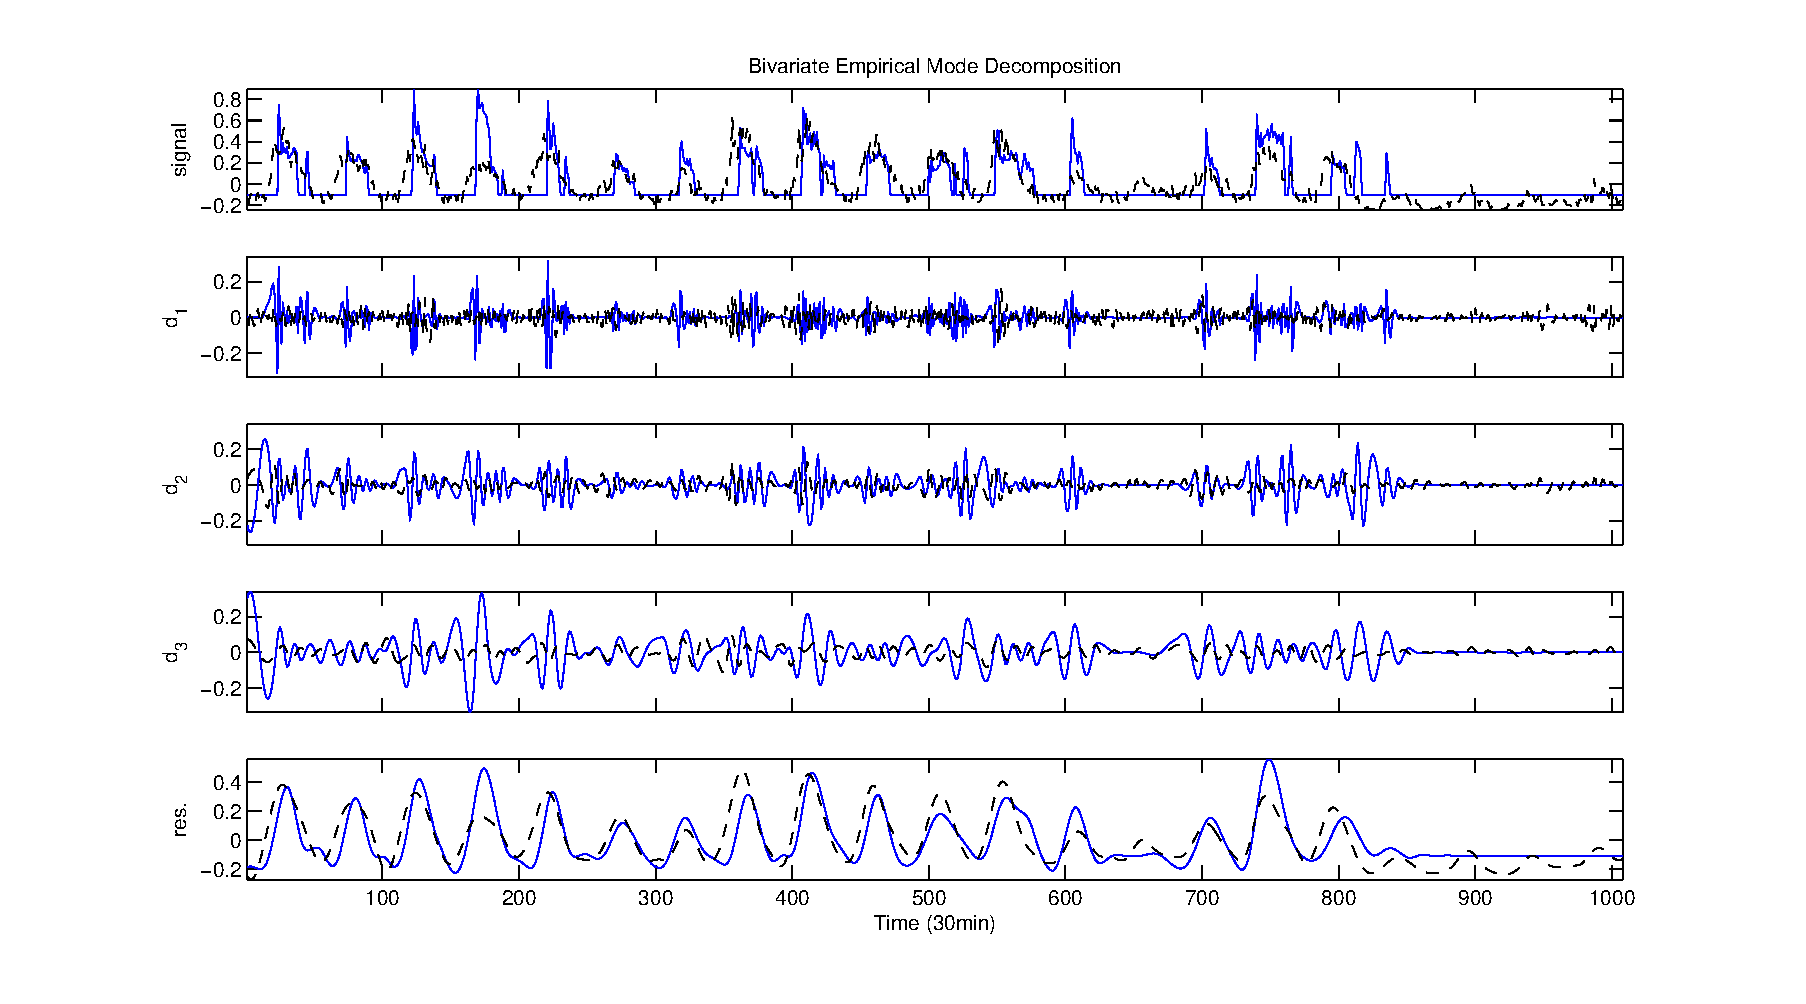
\includegraphics[width=\textwidth]{img/emd_25_41}}
 \caption{Empirical Mode Decomposition}
 \label{fig:raw}
\end{figure*}

\newpage
